%!TEX root = Qualificacao.tex

\section{Randomized Model Structure Selection}%
\label{sec:ramss}

% COMTEMP \todo[inline]{Coloquei o RaMSS por enquanto nesta seção, mas estou querendo colocar em um capítulo a parte. Só mencioná-lo na seção anterior como método de seleção de estrutura. No capítulo a parte colocarei uma introdução sobre métodos estatísticos e teria ainda espaço para exemplos de aplicação do RaMSS para identificação de sistemas (processos). Mai a frente abordaria o uso para identificação de controladores.} 

% O método RaMSS, apresenta uma abordagem alearorizada para escolha de uma estrutura de modelo adequada por meio da amostragem de modelos de um conjunto de modelos $\mathscr{M}$.
The RaMMS method presents a randomized approach for choosing an appropriate model structure by sampling models from a set of models $\mathscr{M}$.
% Introduzido por \cite{falsone2014} e aperfeiçoado em \cite{falsone2015}, o método realiza a tarefa de seleção de estrutura de maneira probabilística que, apesar do caráter aleatório, evita a busca exaustiva necessária para analisar todos os regressores do conjunto de regressores candidatos, definido por $\mathscr{R}$,
Introduced by \cite{falsone2014} and improved in \cite{falsone2015}, the method performs the task of  structure selection in a probabilistic way that, despite the random behavior, avoids the exhaustive search necessary to analyze all the possible models in the set of candidate regressors, defined by $\mathscr{R}$,
% COMTEMP \todo{tentar colocar isso (a definição do conjunto) de uma maneira mais formal (fórmula).} 
% que seria necessário ao se utilizar força bruta em uma estratégia puramente Monte Carlo.
that would be needed when using brute force in a purely Monte Carlo strategy.

% O método procura iterativamente pelo melhor subconjunto de regressores no conjunto $\mathscr{R}$ visando maximizar a acurácia da predição do modelo segundo um índice definido. Isto é feito através de modelos candidatos, subconjuntos de $\mathscr{M}$, construídos a partir de regressores amostrados do conjunto $\mathscr{R}$ com a probabilidade de escolha dada por uma função de probabilidade estimada chamada de RIP (\textit{Regressor Inclusion Probability})
Considering a set of all possible models formed by $\mathscr{R}$, named universe set and represented by $\mathscr{U}$, the method iteratively searches for the best subset of regressors in the $\mathscr{R}$ set in order to maximize the accuracy of the model's prediction according to a defined index. This is done by a set of candidate models, defined as $\mathscr{M} \in \mathscr{U}$, built from regressors sampled from the $\mathscr{R}$ set with a probability of choice given by an estimated probability function called RIP (\textit{Regressor Inclusion Probability}).

% Uma vez escolhido um modelo candidato, este é avaliado de acordo com algum critério de desempenho e os RIP são atualizados. A cada iteração, $N_p$ modelos são tomados de $\mathscr{M}$ e índices de desempenho são calculados para a atualização dos RIP.
Once a candidate model is chosen, it is evaluated according to some performance criteria and the RIPs are updated. At each iteration, $N_p$ models are taken from $\mathscr{U}$ set and performance indexes are calculated for updating the RIPs.
% Estes índices são, em geral,  baseados no MSPE, MSSE ou uma combinação dos dois, e são usados para calcular um índice médio de desempenho do regressor avaliado.

These indexes are, in general, based on the MSPE, MSSE or a combination of the two, and are used to calculate an average performance index $\mathcal{I}$ of the evaluated regressor.
% Assumindo um conjunto $\mathscr{M}$ de $N_p = \dim(\mathscr{M})$ modelos em que alguns contêm o $j$-ésimo regressor, um índice que mensura o \textit{desempenho médio do regressor}, que pode ser usado no cálculo do RIP é definido como
Assuming a set $\mathscr{M}$ of $N_p = \dim(\mathscr{M})$ models, where some contain the $j$-th regressor (and others possibly not), an index that measures the \textit{average performance of the regressor}, which can be used in calculating the RIP is defined as
\begin{align}
   \mathcal{I}_j &= \mathcal{I}_j^+ - \mathcal{I}_j^- \nonumber\\
      % &= \E[\mathcal{J}^{+}_{j}] - \E[\mathcal{J}^{-}_{j}]
      &= \E[\mathcal{J}(\mathscr{M})|\phi_j \in \mathscr{M}] - \E[\mathcal{J}(\mathscr{M})|\phi_j \notin \mathscr{M}],
\label{eq:desMedioReg}
\end{align}
% COMTEMP \todo{decidir aqui: usar $\mathscr{M}$ ou  $ \mathscr{R}$ -- eq. \eqref{eq:desMedioReg}.}
% sendo $j = 1,\ \dots,\ m$, em que  $m = \dim{(\mathscr{R})}$ é o número de regressores considerados, $\mathcal{J}(\mathscr{M})$ representa o vetor contendo os índices de desempenho para os modelos escolhidos, $\mathscr{M}$ é o conjunto de regressores candidatos, $\phi_j$ o $j$-ésimo regressor e $\E[\cdot]$ é o operador de esperança matemática\footnote{Caso o evento condicional tenha probabilidade nula de ocorrer, a esperança é assumida nula.}. Desta forma, o índice de desempenho $\mathcal{I}_j$ compara o desempenho médio dos modelos contendo o $j$-ésimo regressor ($ \mathcal{I}_j^+$) com o desempenho dos modelos que não contêm este mesmo regressor ($ \mathcal{I}_j^+$).
being $j = 1,\ \dots,\ m$, where $m = \dim{(\mathscr{R})}$ is the number of regressors considered, $\mathcal{J}(\mathscr{M})$ represents the vector containing the performance indexes for the chosen models, $\mathscr{M}$ is the set of candidate regressors, $\phi_j$ the $j$-th regressor and $\E[\cdot]$ is the operator of mathematical expectation\footnote{If the conditional event has zero probability of occurring, expectation is assumed to be null.}. Thus, the performance index $\mathcal{I}_j$ compares the average performance of models containing the $j$-th regressor ($ \mathcal{I}_j^+$) with the performance of models that do not contain this same regressor ($ \mathcal{I}_j^+$).
% Como em geral a esperança matemática da equação \eqref{eq:desMedioReg} não pode ser calculada de forma analítica, esta é, na prática, feita por estimação, tomando modelos do modelo universo $\mathscr{U}$ e calculando a média amostral, resultando em
As, in general, the mathematical expectation of the equation \eqref{eq:desMedioReg} cannot be calculated analytically, this is done, in practice, by estimation, taking models from the universe model $\mathscr{U}$ set and calculating the sample mean, resulting in
\begin{equation}
   \mathcal{I}^+_j = \frac{1}{n_j^+}\sum_{i \in \mathscr{M}_j^+}\mathcal{J}^{+}_{i} \qquad \text{e} \qquad \mathcal{I}^-_j = \frac{1}{n_j^-}\sum_{i \in \mathscr{M}_j^-}\mathcal{J}^{-}_{i},
\label{eq:avgRefPerf}
\end{equation}

% onde $ \mathscr{M}^+_j \subset \mathscr{M}$ e $ \mathscr{M}^+_j \subset \mathscr{M}$, representam os conjuntos de todos os modelos que, respectivamente, contêm e não contêm o $j$-ésimo regressor $\phi_j$, com $n_j^+ = \dim \mathscr{M}^+_j $ e $n_j^- = \dim \mathscr{M}^-_j$. Os termos $\mathcal{J}^{+}_{i}$ e  $\mathcal{J}^{-}_{i}$ representam os respectivos índices de desempenho para os casos que contêm e que não contêm $\phi_j$.

where $ \mathscr{M}^+_j \subset \mathscr{M}$ and $ \mathscr{M}^+_j \subset \mathscr{M}$, represent the sets of all models that, respectively, contain and do not contain the $j$-th regressor $\phi_j$, with $n_j^+ = \dim \mathscr{M}^+_j $ and $n_j^- = \dim \mathscr{M}^-_j $. The terms $\mathcal{J}^{+}_{i}$ and $\mathcal{J}^{-}_{i}$ represent the respective performance indexes for cases that contain and do not contain $\phi_j$.



% Assumindo que o modelo real definido por $f^*$, o qual se deseja encontrar, pertence ao conjunto de todas as possíveis estruturas (conjunto universo) $\mathscr{M}$, deve ser possível achar este modelo explorando o conjunto de modelos $\mathscr{M}$ e tomando os modelos com melhor desempenho.  O problema de se achar o modelo real em função de um índice pode ser representado por
Assuming that the actual model, defined by $f^*$, belongs to the set of all possible structures (universe set) $\mathscr{U}$, it must be possible to find this model by exploring the set of models $\mathscr{M}$ and taking the models with the best performance. The problem of finding the real model as a function of an index can be represented by
\begin{equation}
   f^* = \argmax_{\tilde{f} \in \tilde{\mathscr{U}}} \mathcal{J}(\tilde{f}),
\label{eq:fStar}
\end{equation}
% onde $ \mathcal{J}$ é algum\footnote{A definição de $\mathcal{J}$ adotada na proposta original do RaMSS é apresentada mais adiante no texto (vide eqs. \ref{eq:Jp} a \ref{eq:Jcal}). } índice de desempenho calculado para os modelos candidatos $\tilde{f}$ tomados do conjunto universo não redundante  $\tilde{\mathscr{M}} \subset{\mathscr{M}}$\footnote{Note que no conjunto universo é comum o aparecimento de modelos redundantes, oev  seja, modelos similares que não incluem termos estatisticamente relevantes. Na prática é comum que estes sejam removidos e a amostragem seja realizada em um conjunto reduzido do modelo universo, definido por $\tilde{\mathscr{M}} \subset \mathscr{M}$.}, ou   mesmo por $ \mathscr{M}$.
where $ \mathcal{J}$ is some\footnote{The definition of $\mathcal{J}$ adopted in the original proposal of RaMSS is presented later in the text (see eqs. \ref{eq:Jp} a \ref{eq:Jcal}). } performance index calculated for candidate models $\tilde{f}$ taken from the non-redundant universe set $\tilde{\mathscr{U}} \subset{\mathscr{U}}$\footnote {Note that in the universe set it is common for redundant models to appear, ie, similar models that do not include statistically relevant terms. In practice, it is common for these to be removed and sampling to be performed on a reduced set of the universe model, defined by $\tilde{\mathscr{U}} \subset \mathscr{U}$.}, or even by $ \mathscr{U}$.


% No sentido de achar a estrutura correta do modelo, ou seja $ f^*$, o algoritmo RaMSS amostra $N_p$ modelos de $ \mathscr{M}$, calcula o desempenho $\mathcal{J}(\tilde{f})$ para cada modelo candidato $\hat{f}_{i}$, com $i=1,\ \dots,\ N_p$ e estima a média sobre todos os modelos que envolvem o regressor $\phi_j$. Isto é feito para cada um dos $m=\dim(\mathscr{R})$ regressores do conjunto $\mathscr{R}$ de regressores candidatos.
In order to find the correct model structure, i.e. $ f^*$, the RaMSS algorithm samples $N_p$ models from $ \mathscr{U}$, calculates the performance index $\mathcal{J}(\tilde{f})$ for each candidate model $\hat{f}_{i}$, with $i=1,\ \dots,\ N_p$ and estimates the average over all models involving the $\phi_j$-th regressor. This is done for each of the $m=\dim(\mathscr{R})$ regressors of the $\mathscr{R}$ set of regressors.

% Considerando que o índice de desempenho $\mathcal{J}$ em \eqref{eq:fStar} tenha valores no intervalo $[0,\ 1]$, i.e.  $ \mathcal{J}(\tilde{f}) \in \R : \mathcal{J}(\tilde{f}) \in [0,\ 1] $
Considering that the performance index $\mathcal{J}$ in \eqref{eq:fStar} has values in the $[0,\ 1]$ range, i.e. $ \mathcal{J}(\tilde{f}) \in \R : \mathcal{J}(\tilde{f}) \in [0,\ 1] $
\todo{Confirmar isso aqui}, 
% o valor esperado de $\mathcal{J}$,
% seu valor esperado, considerando $ \mathcal{P}$ a distribuição de probabilidade ao se escolher o regressor $\phi_j$ como variável aleatória $\mathscr{M}$ na realização de uma amostra de modelo em  $ \tilde{\mathscr{M}}$, será dado por
its expected value, considering the probability distribution  $ \mathcal{P}$ and a random variable $\Phi \equiv \tilde{\mathscr{M}}$ that corresponds to a realization a model sample in $ \tilde{\mathscr{U}}$, will be given by
\begin{equation}
  \E[\mathcal{J}] = \sum_{\tilde{f}\in \tilde{\mathscr{U}}} \mathcal{J}(\tilde{f})\mathcal{P}(\mathscr{U}=\tilde{f})
\label{eq:espJ}
\end{equation}

% Se $\mathcal{P}$ é variado sobre todas as possíveis distribuições em $\tilde{\mathscr{U}}$, o máximo de \eqref{eq:espJ} é obtido ao se concentrar toda a massa de probabilidade no modelo mais adequado. Com isso, a solução do problema de otimização pode é obtida por
If $\mathcal{P}$ is varied over all possible distributions in $\tilde{\mathscr{U}}$, the maximum of \eqref{eq:espJ} is obtained by concentrating the entire probability mass on the most appropriate model. With that, the solution to the optimization problem can be obtained by
\begin{equation}
   \mathcal{P}^* = \argmax_{\Phi\in  \tilde{\mathscr{U}}} \E\left[ \mathcal{J}(\Phi)  \right]   
\label{eq:Pargmax}
\end{equation}
% e é tal que $\mathcal{P}=1$. Assim, resolvendo \eqref{eq:Pargmax} seleciona-se o modelo mais adequado, ou modelo real $f^*$, com a mesma solução de \eqref{eq:fStar}.
and it's such that $\mathcal{P}=1$. Thus, by solving \eqref{eq:Pargmax}, the most appropriate model, or real model $f^*$, is selected with the same solution as \eqref{eq:fStar}.

% O método RaMSS estima $\mathcal{P}$ e, consequentemente, o melhor modelo como se segue. A cada iteração, $N_p$ modelos candidatos são montados a partir de $m$ regressores candidatos. A escolha de cada regressor $\phi_j$ componente de um modelo candidato é feita a partir de um processo de Bernoulli, por uma variável aleatória associada a cada regressor  $\phi_j$ tal que
The RaMSS method estimates $\mathcal{P}$ and, consequently, the best model as follows. At each iteration, $N_p$ candidate models are assembled from $m$ candidate regressors. The choice of each $\phi_j$ regressor component of a candidate model is made based on a Bernoulli process, by a random variable associated with each $\phi_j$ regressor such that
\begin{equation}
   \rho \approx \text{Be}(\mu_j),
\label{eq:bernulli}
\end{equation}
% onde possíveis resultados são: 1, com probabilidade (de sucesso) $\mu_j$ de ocorrer; e 0, com probabilidade $(1-\mu_j)$; sendo $\mu_j \in [0,\ 1]$,  com $ j=1, \dots, m$ e $m$ o número de regressores candidatos.
where possible results are: $\rho=1$, with $\mu_j$ probability (of success) to occur; and $\rho=0$, with probability $\mu_j$; where $\mu_j \in [0,\ 1]$, with $ j=1, \dots, m$ and $m$ the number of candidate regressors.
% Caso $\rho=1$, o regressor  $\phi_j$ estará presente no modelo candidato construído, caso contrário, não.
If $\rho=1$, the $\phi_j$ regressor will be present in the candidate model built, otherwise, no.

% Assume-se que variáveis aleatórias $\rho_j$ são independentes\footnote{Apesar de existirem resultados na literatura \citep{bianchi2016} sugerindo que uma abordagem utilizando distribuição Bernoulli condicionada e multivariada pode resultar em melhorias na acurácia do processo de seleção de modelos, um procedimento inicial adotado neste trabalho considera independência.} e define-se um vetor $\bm{\mu} = [\mu_1,\ \mu_2,\ \dots,\ \mu_m]^T$ como o vetor de \textit{Probabilidade de Inclusão de Regressor} (RIP). Note que o RIP, ou $\vmu$ é quem dita a distribuição de probabilidade  $ \mathcal{P}$ sobre os modelos em $\tilde{\mathscr{M}}$ (ou $\mathscr{M}$), ou seja, dado um $\bm{\mu}$ conhecido, a probabilidade de se obter um modelo de estrutura $\tilde{f}$ em qualquer subconjunto de $n_\theta$ regressores será
It is assumed that $\rho_j$ random variables are independent \footnote{Although there are results in the literature \citep{bianchi2016} suggesting that an approach using conditioned and multivariate Bernoulli distribution may result in improvements in the accuracy of the model selection process, an initial procedure adopted in this work considers independence.} and a $\bm{\mu} = [\mu_1,\ \mu_2,\ \dots,\ \mu_m]^T$ vector is defined as the vector of \textit{Probability of Inclusion of Regressor} (RIP). Note that the RIP, or $\vmu$, is the one that dictates the $ \mathcal{P}$ probability distribution on the models in $\tilde{\mathscr{U}}$ (or $\mathscr{U}$), that is, given a known $\bm{\mu}$, the probability of obtaining a $\tilde{f}$ structure model in any subset of $n_\theta$ regressors is
\begin{equation}
   \mathcal{P}(\tilde{f}) = \prod_{j:\phi_j \in \tilde{f}}^{n_{\theta}} \mu_j \prod_{j:\phi_j \notin \tilde{f}}^{m-n_{\theta}} (1-\mu_j),
\label{eq:distProbf_til}
\end{equation}
to any $ \tilde{f} \in \tilde{\mathscr{U}}$.

% O procedimento é executado de modo que a cada iteração os regressores são escolhidos de acordo com o processo de Bernoulli, onde a probablilidade de escolha $\mu_j$ de cada regressor $\phi_j$ é representada pelo vetor de RIP. O vetor de RIP, $\bm{\mu}$ é refinado por sucessivas iterações de uma regra de atualização definida como
The procedure is performed so that at each iteration the regressors are chosen according to the Bernoulli process, where the probability of choosing $\mu_j$ for each $\phi_j$ regressor is represented by the RIP vector. The RIP vector, $\bm{\mu}$ is refined by successive iterations of an update rule defined as
\begin{equation}
   \mu_j(i+1) = \mu_j(i) + \gamma \mathcal{I}_j,
\label{eq:RIPupdate}
\end{equation}
% onde $\gamma$ é um parâmetro de projeto, $I_j$ o índice de desempenho definido em \eqref{eq:desMedioReg} e $i$ o índice da iteração do algoritmo.
where $\gamma$ is a project parameter, $\phi_j$ the performance index defined in \eqref{eq:desMedioReg} and $i$ the index of the algorithm's iteration.

% \vspace{2cm} \hrulefill

% Depois de algumas iterações é esperado que os desempenhos médios dos modelos que contém os regressores certos fiquem significantemente maiores que os que não contém, fazendo com que os regressores ``corretos'' sejam mais prováveis de serem incluídos no modelo final. O método não garante que $ \bm{\mu}$ será limitado. Para evitar que os valores do RIP cresçam, ou decresçam indefinidamente, uma saturação dos elementos em uma faixa com valor mínimo maior ou igual a 0, e máxima, menor ou igual a 1, é aplicada pelo algoritmo.
After a few iterations, it is expected that the average performances of the models containing the right regressors will be significantly higher than those that do not, making the correct regressors more likely to be included in the final model. The method does not guarantee that $ \bm{\mu}$ will be limited. To prevent the RIP values from increasing, or decreasing indefinitely, a saturation of the elements in a range with a minimum value greater than or equal to 0, and a maximum value less than or equal to 1, is applied by the algorithm.

% O parâmetro de projeto $\gamma$, de  \eqref{eq:RIPupdate} é escolhido de forma a controlar a velocidade de convergência. Valores maiores tendem a levar a uma convergência mais rápida mas pode também levar a não convergência do método. Para lidar com este problema de convergência, \cite{falsone2015} propõem um parâmetro adaptativo, dado por
The project parameter $\gamma$, from \eqref{eq:RIPupdate} is chosen in order to control the convergence speed. Larger values tend to lead to faster convergence but it can also lead to non-convergence of the method. To deal with this convergence problem, \cite{falsone2015} proposes an adaptive parameter, given by
\begin{equation}
   \gamma = \frac{1}{10(\mathcal{J}_{\max}- \bar{\mathcal{J}}) + 0.1}, 
\label{eq:gamma}
\end{equation}
% onde $\mathcal{J}_{\max}$ representa o índice de desempenho do melhor modelo e $\bar{\mathcal{J}}$ representa o índice de desempenho médio na iteração corrente.
where $\mathcal{J}_{\max}$ represents the performance index of the best model and $\bar{\mathcal{J}}$ represents the average performance index in the current iteration.
% A proposta do passo adaptativo é de que, se $\bar{\mathcal{J}}$ está longe do melhor índice de desempenho, $\gamma$ é feito pequeno de modo a compensar a grande variância provável daquela população de modelos. Porém, se  $\bar{\mathcal{J}}$ é próximo de $\mathcal{J}_{\max}$, os modelos amostrados têm baixa variância de desempenho, o que indica que o RIP deve ser atualizado em maior valor.
The purpose of the adaptive step is that, if $\bar{\mathcal{J}}$ is far from the best performance index, $\gamma$ is made small in order to compensate for the large probable variance of that model population. However, if $\bar{\mathcal{J}}$ is close to $\mathcal{J}_{\max}$, the sampled models have low performance variance, which indicates that the RIP should be updated to a greater value.

% O método RaMSS, como apresentado originalmente pelos autores, utiliza como base para o cálculo do índice de desmpenho $\mathcal{J}$, grandezas relacionadas ao MSPE e ao MSSE, definidos na seção \ref{sec:model_validation}. O índice de desempenho médio é calculado como um valor exponencial destes índices ponderados por um ganho $K$, utilizado como parâmetro de projeto. Desta forma tem-se,
The RaMSS method, as originally presented by the authors, uses as basis for calculating the performance index $\mathcal{J}$, quantities related to MSPE and MSSE, defined in the Section \ref{sec:model_validation}. The average performance index is calculated as an exponential value of these indices weighted by a $K$ gain, used as a design parameter. This way,
\begin{align}
  \mathcal{J}_p = e^{-K\cdot MSPE}, \label{eq:Jp} \\
  \mathcal{J}_s = e^{-K\cdot MSSE}. \label{eq:Js}
\end{align}
% Note que $\mathcal{J}_p$ e $\mathcal{J}_s$ terão valores no intervalo $[0 \ 1]$, onde valores próximos a 1 correspondem a um melhor desempenho, e próximos a 0, a piores desempenhos.
Note that $\mathcal{J}_p$ and $\mathcal{J}_s$ will have values in the $[0 \ 1]$ range, where values close to 1 correspond to better performance, and close to 0, worse performance. The $K$ parameter defines the sensitivity of the performance index, where the difference between models is amplified to values greater than $K$.

% O valor final de $\mathcal{J}$ é calculado como
The final value of $\mathcal{J}$ is calculated as
\begin{equation}
  \mathcal{J} = \alpha \mathcal{J}_s + (1-\alpha)\mathcal{J}_p
\label{eq:Jcal}
\end{equation}
% onde $\alpha \in [0 \ 1]$ é um parâmetro definido pelo projetista. O parâmetro $K$ define a sensibilidade do índice de desempenho, onde a diferença entre modelos é amplificada para valores maiores de $K$.
where $\alpha \in [0 \ 1]$ is a parameter defined by the designer. 

% COMTEMP \todo[inline, color=red]{Continuar aqui!??}

% TODO: [DONE] {Colocar aqui sobre $\mathcal{J}$, como é definido, etc.}

% Passadas algumas iterações o espera-se que vetor de RIP, $\bm{\mu}$, convirja para uma distribuição de equilíbrio. O modelo final será o modelo correto esperado do sistema e será composto pelos regressores associados aos RIP com valores maiores que certo limiar definido pelo projetista. Assumindo-se que o modelo real $f^* \in \tilde{\mathscr{M}}$, este limiar em geral é ajustado para um valor próximo a 1.
After a few iterations, the RIP vector, $\bm{\mu}$, is expected to converge to an equilibrium distribution. The final model will be the correct model expected from the system and will consist of regressors associated with RIPs with values greater than a certain threshold defined by the designer. Assuming that the real model $f^* \in \tilde{\mathscr{U}}$, this threshold is generally set to a value close to 1.

% O pseudo-código para o método RaMSS descrito é apresentado no Algorithm \ref{alg:RaMSS}. Na sequência é apresentado  um exemplo para identificação de sistema utilizando o  método.
The pseudo-code for the described RaMSS method is presented in Algorithm \ref{alg:RaMSS}. Following is an example for system identification using the method.
    % \For(\tcp*[f]{Start Policy Improvement}){each $\vx_k \in \Omega_k$}

\begin{algorithm}[htpb]
  \caption{RaMSS algorithm}\label{alg:RaMSS}
  $\bm{y},N_p,m,\mu_{\min},\mu_{\max},K,\mathscr{M}=\{\phi_{1},\dots,\phi_{m}\}$ \\
  \While{$iter < iter_{\max}$} 
   {
     $ \bm{\mu} \gets \bm{\mu}_0$
     \For(\tcp*[f]{Model Sampling}){$i=1:N_p$}
      {
         $\tau \gets 0$ \\
         $\bm{\psi}(k) \gets [\ ]$ \tcp*[f]{Initialize model} \\
         \For{$i=1:m$}
         {
           $r_j \gets \text{Be}(\mu_j)$ \tcp*[f]{Sample from a Bernoulli distribution}\\
            \If{$r_j = 1$}
            {
            $\bm{\psi}(k) \gets \begin{bmatrix} \bm{\psi}^T(k) & \phi_j \end{bmatrix}^T $ \\
            $\tau \gets \tau + 1$ \\
            }
         }
         \For{$h=1:\tau$}
         {
           $\tilde{\bm{\psi}}(k) \gets \text{non-redundant}(\bm{\psi(k)})$ \tcp*[f]{Remove redundant terms}\\
         }
         $\hat{\bm{y}} \gets \text{Predict}(\tilde{\bm{\psi}}(k))$ \\
         $\mathcal{J}_i \gets e^{-K\cdot MSPE(\bm{y},\bm{\hat{y}})} $
      }
      \For(\tcp*[f]{RIP Update}){$j=1:m$}
      {
         $\mathcal{J}^{+} \gets 0$; $ \mathcal{J}^{-}$; $n^{+} \gets 0$; $n^{-} \gets 0$; \\
         \For{$i=1:N_p$}
         {
            \If{$\phi_j(k) \in \tilde{\bm{\psi}}(k)$}
            {
               $\mathcal{J}^{+} \gets \mathcal{J}^{+} + \mathcal{J}_i$ \\
               $n^{+} \gets n^{+} + 1$
            } \Else
            {
               $\mathcal{J}^{-} \gets \mathcal{J}^{-} + \mathcal{J}_i$ \\
               $n^{-} \gets n^{-} + 1$
            }
            $\mathcal{I}_j \gets \left( \frac{\mathcal{J}^{+}}{\max(n^+,1)} \frac{\mathcal{J}^{-}}{\max(n^-,1)} \right) $ \\
         $\mu_j \gets \mu_j + \gamma \mathcal{I}_j$ \\
         $\mu_j \gets \max \left( \min(\mu_j, \mu_{\max}), \mu_{\min} \right) $ \\
         }
      }
   }
\end{algorithm}%[H]

\begin{exmp}[Idendificação de um modelo não-linear utilizando o RaMSS]
  \label{ex:varHeater}
  % Como exemplo ilustrativo da utilização do algoritmo RaMSS na escolha de estrutura e identificação de sistemas é usado um modelo de um pequeno aquecedor elétrico, com dissipação variável. A variação da dissipação é resultado do acionamento de um ventilador. O sinal de entrada é a tensão elétrica aplicada ao aquecedor e a saída é o sinal amplificado de um termopar. Mais detalhes sobre este modelo podem ser encontrados em \citep{aguirre2015}, seção 16.6.

  % Como exemplo ilustrativo da utilização do algoritmo RaMSS na escolha de estrutura e identificação de sistemas é usado um modelo não linear fornecido em \cite{baldacchino2013}, dado por:
  As an illustrative example of the use of the RaMSS algorithm in the structure selection, consider a nonlinear model provided in \cite{baldacchino2013}, given by:
  \begin{equation}
    y(k) = 0.7y(k-1)u(k-2) - 0.5y(k-2) + 0.6u^2(k-2) - 0.7y(k-2)u^2(k-2) + e(k)
  \label{eq:}
  \end{equation}
  % sendo o sinal de excitação $u(k)$ adotado como um sinal com distribuição uniforme entre -1 e 1, i.e. $u(k) \sim \mathcal{U}(-1,1) $ e um ruído branco gaussiano $e(k)$ com distribuição gaussiana com variância 0.02 e média nula, i.e. $e(k) \sim \mathcal{N}(0,0.02)$.
  where $u(k)$ is the excitation signal, adopted as a signal with uniform distribution between -1 and 1, i.e. $u(k) \sim \mathcal{U}(-1,1) $ and $e(k)$ is a white Gaussian noise with a variance of 0.02  and zero mean, i.e. $e(k) \sim \mathcal{N}(0,0.02)$.

  % O algoritmo \ref{alg:RaMSS} é aplicado para um numero máximo de 100 iterações.
  The Algorithm \ref{alg:RaMSS} algorithm is applied for a maximum number of 100 iterations.
  % A cada iteração, um total de $N_p = 100$ modelos são escolhidos para o cálculo dos índices de usados na atualização dos RIPs.
  At each iteration, a total of $N_p = 100$ models are chosen to calculate the indexes used in the RIPs update.
  % A Figura \ref{fig:ex31_rips} mostra o comportamento típico dos RIPs durante as atualizações. Nota-se que o regressor $u^2(k-2)$ converge rapidamente, em aproximadamente 14 iterações, seguido pelos regressores  $y(k-2)$, $y(k-1)u(k-1)$ e $y(k-2)u^2(k-2)$.
  Figure \ref{fig:ex31_rips} shows a typical behavior of RIPs during updates. Note that the $u^2(k-2)$ regressor converges quickly, in approximately 14 iterations, followed by the $y(k-2)$, $y(k-1)u(k-1)$ and $y(k-2)u^2(k-2)$ regressors.
  \begin{figure}[H]
    \centering
    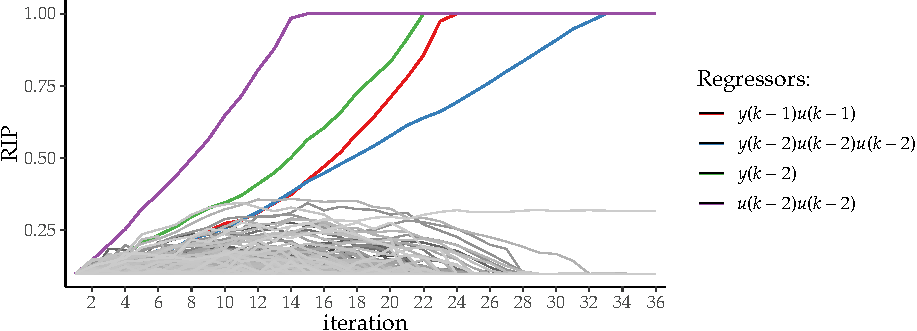
\includegraphics{./Figs/Cap3/ex31_ripsEvol.tex.pdf}
    \caption{Convergence of RIPs considering a particular realization.}
    \label{fig:ex31_rips}
  \end{figure}
  
  % Uma análise mais geral, que leva em conta o comportamento em 100 realizações é mostrado na Figura \ref{fig:ex31_density}. Neste caso observa-se que o comportamento anterior permanece na média, sendo que os regressores $y(k-1)u(k-1)$ e $y(k-2)$ são escolhidos com intervalos próximos, em média.
  A more general analysis, which takes into account the behavior in 100 realizations, is shown in Figure \ref{fig:ex31_density}. In this case it is observed that the previous behavior remains in the average.
  
  \begin{figure}[H]
    \centering
    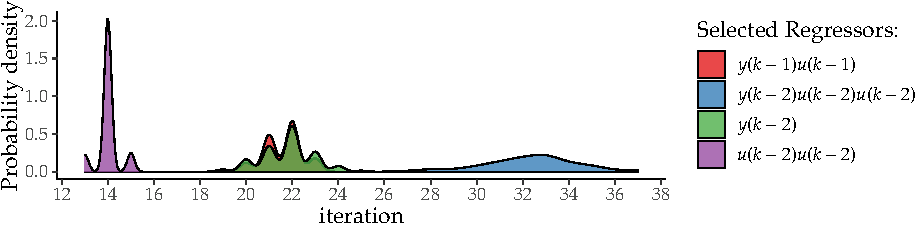
\includegraphics{./Figs/Cap3/ex31_density.tex.pdf}
    \caption{Probability density for convergence of RIPs, considering 100 realizations.}
    % COMTEMP \todo[inline]{Colocar linha de \textit{threshold} na ref{fig:RIPs1}? Mudar cores. Tentar mudar nome dos regressores (índices). Mas com certeza, mudar nomes de y para u.}
    \label{fig:ex31_density}
  \end{figure}

  % Note que os gráficos consideram somente até a 36a iteração. Isto ocorre devido ao critério de parada adotado, que interrompe o procedimento assim que as variações nos RIPs se tornam menor que um certo valor predefinido.
  Note that the graphs only consider up to the 36th iteration. This is due to the adopted stopping criteria, which interrupts the procedure as soon as the variations in the RIPs become less than a certain predefined value.
  % Ressalta-se que em todas as simulações o procedimento parou antes da 100a iteração selecionando exatamente os regressores originais, indicando que há sempre uma convergência para estes valores.
  In all simulations the procedure stopped before the 100th iteration, selecting exactly the original regressors, indicating that there is always a convergence for these values in this exemple.

% Densidade de probabilidade para convergência dos RIPs, considerando-se 100 realizações.
\end{exmp}

